\chapter{Discussion}\label{sec:discussion}

\begin{comment}
The results chapter should simply present the results of applying the methods presented in the method chapter without further ado. This chapter will typically contain many graphs, tables, etc. Sometimes it is natural to discuss the results as they are presented, combining them into a `Results and Discussion' chapter, but more often they are kept separate.

Here you should discuss all aspect of your thesis and project. How did the process work? Which choices did you make, and what did you learn from it? What were the pros and cons? What would you have done differently if you were to undertake the same project over again, both in terms of process and product? What are the societal consequences of your work?
\end{comment}

\section{Collected data}
\todo{Describe what data has been collected}
\todo{Comment on validity/relevance of collected data}
% Write about what we know about the data. In the final thesis, have a more in-depth analysis



\section{Systematic literature review}\label{sec:results-slr}
% Talk about the plans for the SLR for the next semester
% Mention resources, search string, number of results, exclusions
In this section we will present the results we have thus far from our SLR. We will also explain what is missing at this point in time and lay out the road ahead for the upcoming semester, spriing 2025.

\subsection{Study selection}
% Describe the results of the search and selection process, from the number of records identified in the search to the number of studies included in the review, ideally using a flow diagram
Following the selection process outlined in section \ref{sec:slr-selection-process}, we obtained the results as shown in the PRISMA flowchart of figure \ref{fig:prisma-flowchart}.

\begin{figure}[h!]
    \centering
    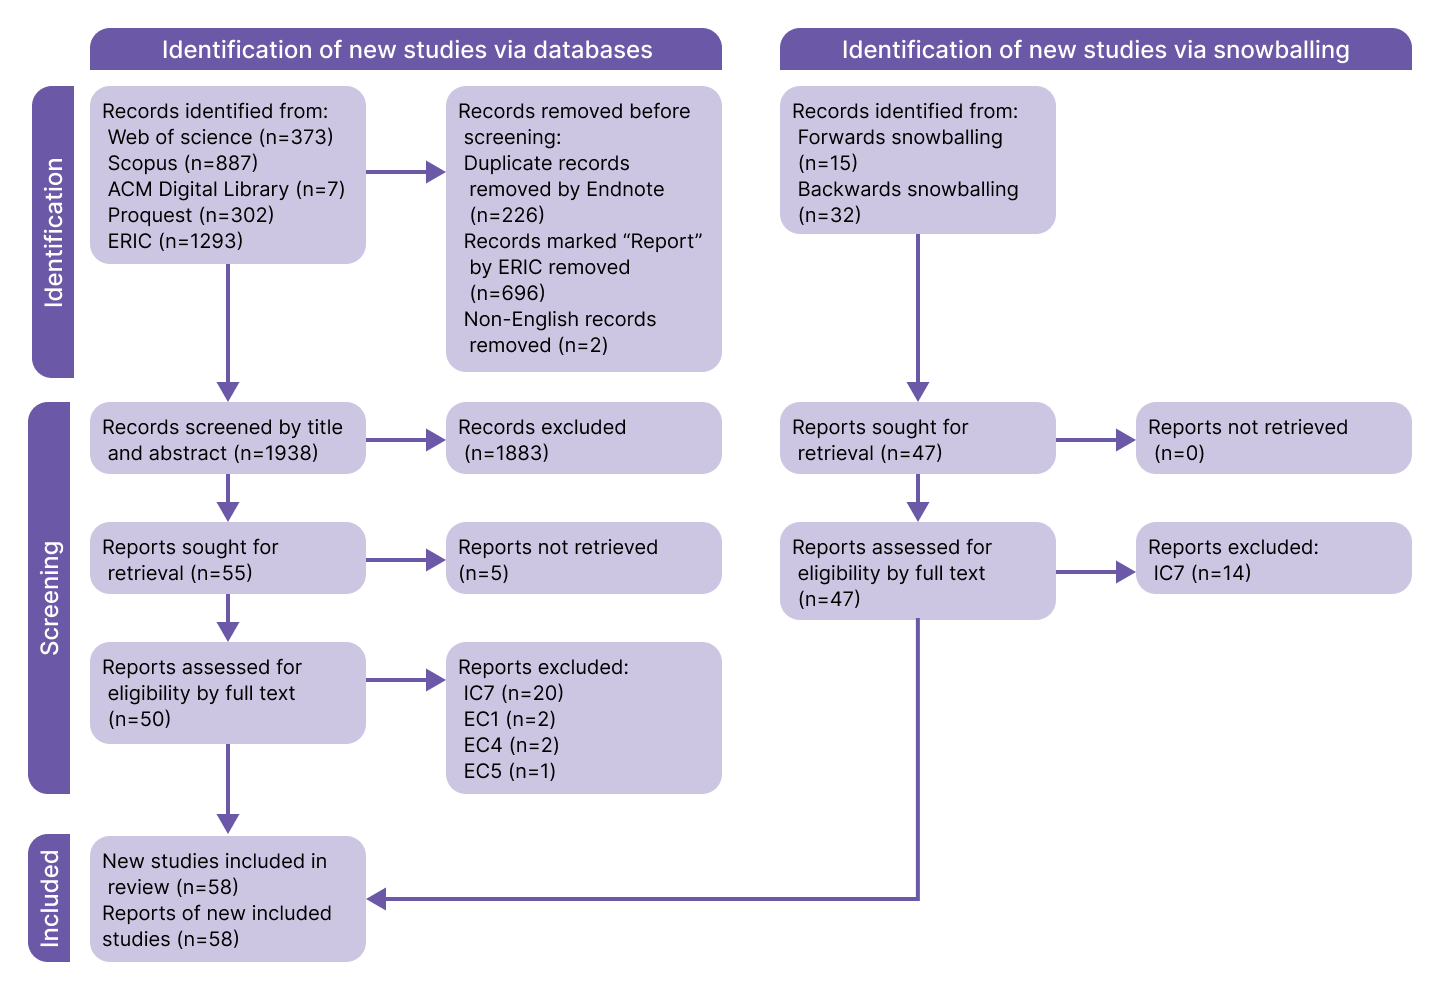
\includegraphics[width=\textwidth]{figures/PRISMA diagram.png}
    \caption{PRISMA flowchart depicting the results of the study selection process.}
    \label{fig:prisma-flowchart}
\end{figure}

When we entered our search query into the five scientific databases and applied the respective filters and limits, we ended up with a total of 2862 papers. 373 of these came from Web of science, 887 from Scopus, only seven from ACM Digital library, 302 from Proquest and 1293 from ERIC. After having exported all the papers to Endnote, we noticed that 696 of the papers coming from ERIC were marked as reports instead of journal articles, despite having set the \textit{Journal articles} filter. These were removed, as we are interested in paper describing new research. After that we used Endnote's built-in functionality to remove duplicates, which resulted in 226 fewer papers. Lastly, two papers were removed that were not in English, leaving us with 1938 papers for screening.

When screening the titles and abstracts, we applied the eligibility criteria. 1883 papers were excluded after this, leaving 55 papers. Five of these did not have full text available. 50 papers were subsequently full text screened and the exclusion reason reported. For the IDs of the eligibility criteria refer to table \ref{tab:eligibilitycriteria}.

We, thereafter, performed an iteration of forwards and backwards snowballing on the 25 papers that were included after full text screening. 15 papers were found through forwards snowballing, which is to say through the papers' citations, and 32 through backwards snowballing, which is to say through the papers' references. Some papers appeared both in citations and references, in which case they are reported as coming from backwards snowballing. Papers that were already found through searching the databases were immediatly excluded as duplicates and not part of the reported statistics in figure \ref{fig:prisma-flowchart}. Snowballing resulted in 47 new papers, of which 14 were excluded due to them not fullfilling inclusion criterion IC7. We were then left with 33 papers from snowballing, with the total count of included papers being 58. These 58 went on to be part of the data extraction process.

While these 58 papers are all published in the period 2015-2024, we have compiled the bar chart in figure \ref{fig:papersbyyear} to get an idea of the papers' timeline. Most of the papers were published in 2019, 2023 and 2020. However, the chart shows no significant trend.

\begin{figure}[h!]
    \centering
    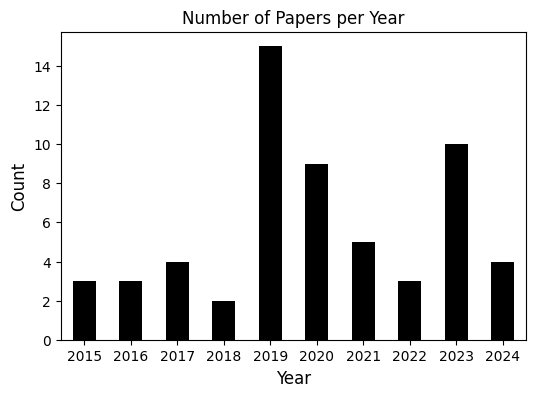
\includegraphics[width=\linewidth]{figures/papers-by-year.png}
    \caption{Distribution of included papers by publication year}
    \label{fig:papersbyyear}
\end{figure}

\subsection{Current status}
As mentioned, the work on the SLR is not completed and will resume in the spring semester 2025, with the aim of publishing it eventually on the side of the master thesis. At this point in time, we have completed the study selection, and we have carried out data extraction for the 58 included papers. The data extraction still requires some work, however. We will in the following attempt to explain the next steps for the SLR.

\begin{enumerate}
    \item \textit{Quality assessment}: The quality of the included papers must be assessed. For this we must develop some quality assessment rules to be applied on all 58 papers. This will ensure that the papers contain sufficient information for our needs and that the results of the studies are truly relevant for our SLR.
    \item \textit{Research questions}: While we have an outline for what data shall be reported in the SLR and an idea of what the SLR should accomplish, we still need to define concrete research questions that can be answered during sythesis of the results.
    \item \textit{Continue data extraction}: We have already extracted data from all 58 papers, but the codes need to be refined further to make the reporting of the data more meaningful and valuable.
    \item \textit{Data synthesis}: After reporting the extracted data, we must make sense of the findings and use the insight to answer our research questions.
    \item \textit{Write the paper}: When we have answered our research questions, the paper itself must be written. This will include explaining the rationale of our SLR, present our research questions and why they are relevant, present the employed SLR methodology, report the results of the paper selection process, report the data from the included papers, answer the research questions, and conclude on what we have achieved with the SLR.
\end{enumerate}

Until now we have been three people working on this SLR. This includes the two of us - in the form of two master students - and a PhD candidate. In the coming semester, the work will mainly be conducted by the PhD candidate while we focus on the master thesis. To perform our experiments on the collected open-text data next semester, we will be dependent on using insights from the SLR as a guide in choosing which AI methods to test, which preprocessing steps and tools may be effective and how different AI methods can be combined to provide more actionable insights from the open-text data.

\subsection{Main findings from papers}
\todo{Describe which AI algorithms have been used, how data was collected and results}

\subsection{Relevant future research} (gaps and limitations)
\todo{What future research is needed in the field?}


\section{Open problems in the domain}




% Keep preliminary RQ as a goal instead of finding a concrete RQ

% \section{Preliminary research question for master thesis}
% \todo{Create a research question for next semester based on the findings}

% Suggestion: How to get actionable insights from students' open-text responses through the use of AI?